\chapter{Unsupervised MGXS Clustering}
\label{chap:methods}


%%%%%%%%%%%%%%%%%%%%%%%%%%%%%%%%%%%%%%%%%%%%%%%%%%%%%%%%%%%%%%%%%%%%%%%%%%%%%%%
\section{Motivation}
\label{sec:chap6-motivate}

\begin{itemize}[noitemsep]
  \item identify metrics of interest - eigenvalue, fission, capture rates
  \item motivate with results for degenerate, null, LNS cases
  \begin{itemize}[noitemsep]
    \item table of eigenvalues
    \item histogram of fission/capture max/mean errors
  \end{itemize}
\end{itemize}


%%%%%%%%%%%%%%%%%%%%%%%%%%%%%%%%%%%%%%%%%%%%%%%%%%%%%%%%%%%%%%%%%%%%%%%%%%%%%%%
\section{A Latent Variable Model for MGXS Clustering}
\label{sec:chap6-latent-model}


%%%%%%%%%%%%%%%%%%%%%%%%%%%%%%%%%%%%%%%%%%%%%%%%%%%%%%%%%%%%%%%%%%%%%%%%%%%%%%%
\section{Overview of Approach}
\label{sec:chap6-overview}

\begin{figure}
  \centering
  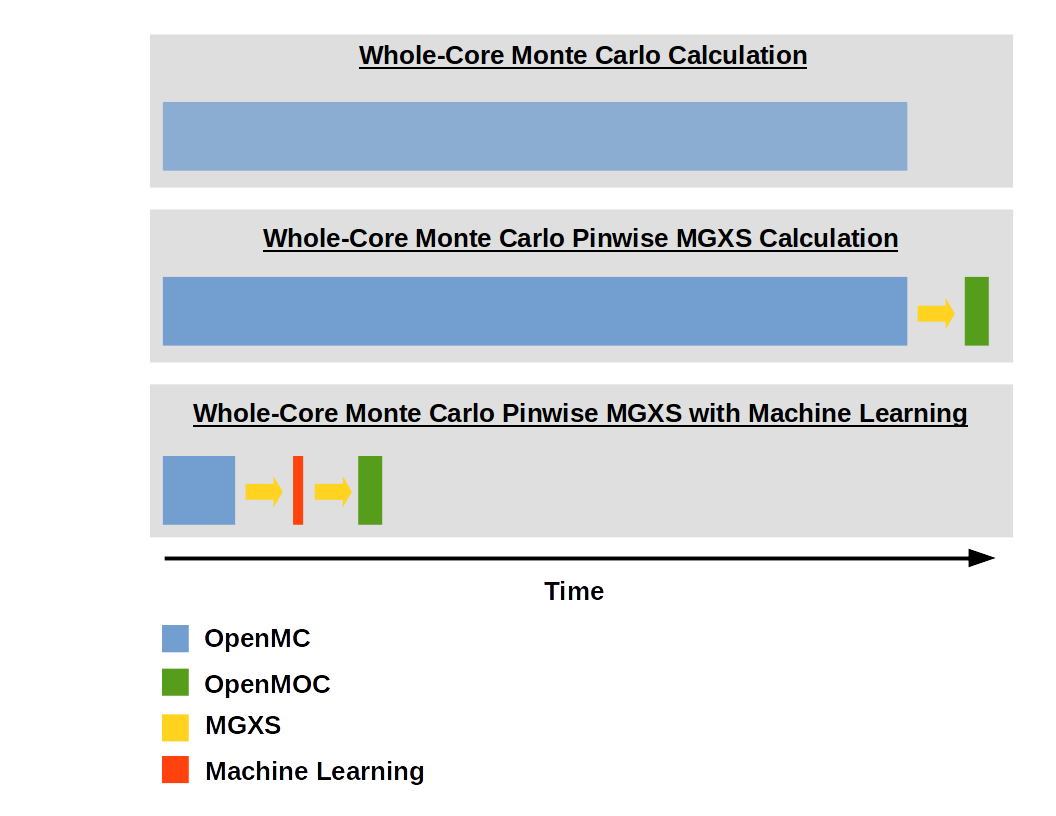
\includegraphics[width=\linewidth]{figures/pipeline/flow-chart}
  \caption{}
\caption[flowchar]{flowchart}
\label{fig:chap6-flow-chart}
\end{figure}



%%%%%%%%%%%%%%%%%%%%%%%%%%%%%%%%%%%%%%%%%%%%%%%%%%%%%%%%%%%%%%%%%%%%%%%%%%%%%%%
\section{Feature Engineering}
\label{sec:chap6-feature-engineer}

%%%%%%%%%%%%%%%%%%%%%%%%%%%%%%
\subsection{Possible Features}
\label{subsec:chap6-feature-select}

%%%%%%%%%%%%%%%%%%%%%%%%%%%%%%
\subsection{Target Selection}
\label{subsec:chap6-feature-select}

%%%%%%%%%%%%%%%%%%%%%%%%%%%%%%%%%%%
\subsection{Feature Transformation}
\label{subsec:chap6-feature-transform}

%%%%%%%%%%%%%%%%%%%%%%%%%
\subsection{Feature Selection}
\label{subsec:chap6-litmus}


%%%%%%%%%%%%%%%%%%%%%%%%%%%%%%%%%%%%%%%%%%%%%%%%%%%%%%%%%%%%%%%%%%%%%%%%%%%%%%%
\section{Approaches to Clustering}
\label{sec:chap6-cluster}

\begin{itemize}[noitemsep]
  \item dataset restrictions
  \begin{itemize}[noitemsep]
    \item \textbf{``pinch'' clustering} - a \textit{single} nuclide/group/reaction triplet
    \item \textbf{``combined'' clustering} - one or more nuclide/group pairs \textit{together}
    \item \textbf{``local'' clustering} - one or more nuclide/group pairs \textit{separately}
  \end{itemize}
  \item clustering algorithms
  \begin{itemize}[noitemsep]
    \item discriminative clustering ($k$-Means++, Agglomerative, etc.)
    \item generative clustering (Gaussian Mixtures, Dirichlet Processes)
  \end{itemize}
  \item ``regression-informed'' clustering
  \begin{itemize}[noitemsep]
    \item use a regressor to predict ``smoothed'' of target variable(s)
    \begin{itemize}[noitemsep]
      \item decision tree regression
      \item ensemble (boosting, random forest) regression
      \item Gaussian Process regression
    \end{itemize}
    \item cluster predictions produced by regressor
    \item advantage is that objective function \textit{may} be more appropriate
  \end{itemize}
\end{itemize}